\chapter{Appendix B}
    \chapterprecishere{
        ``Potentielle citation sans aucun rapport avec le sujet"\par\raggedleft--- \textup{Personne inconnue}, contexte à déterminer
    }
    
    
\begin{figure}[h]
	\centering
	{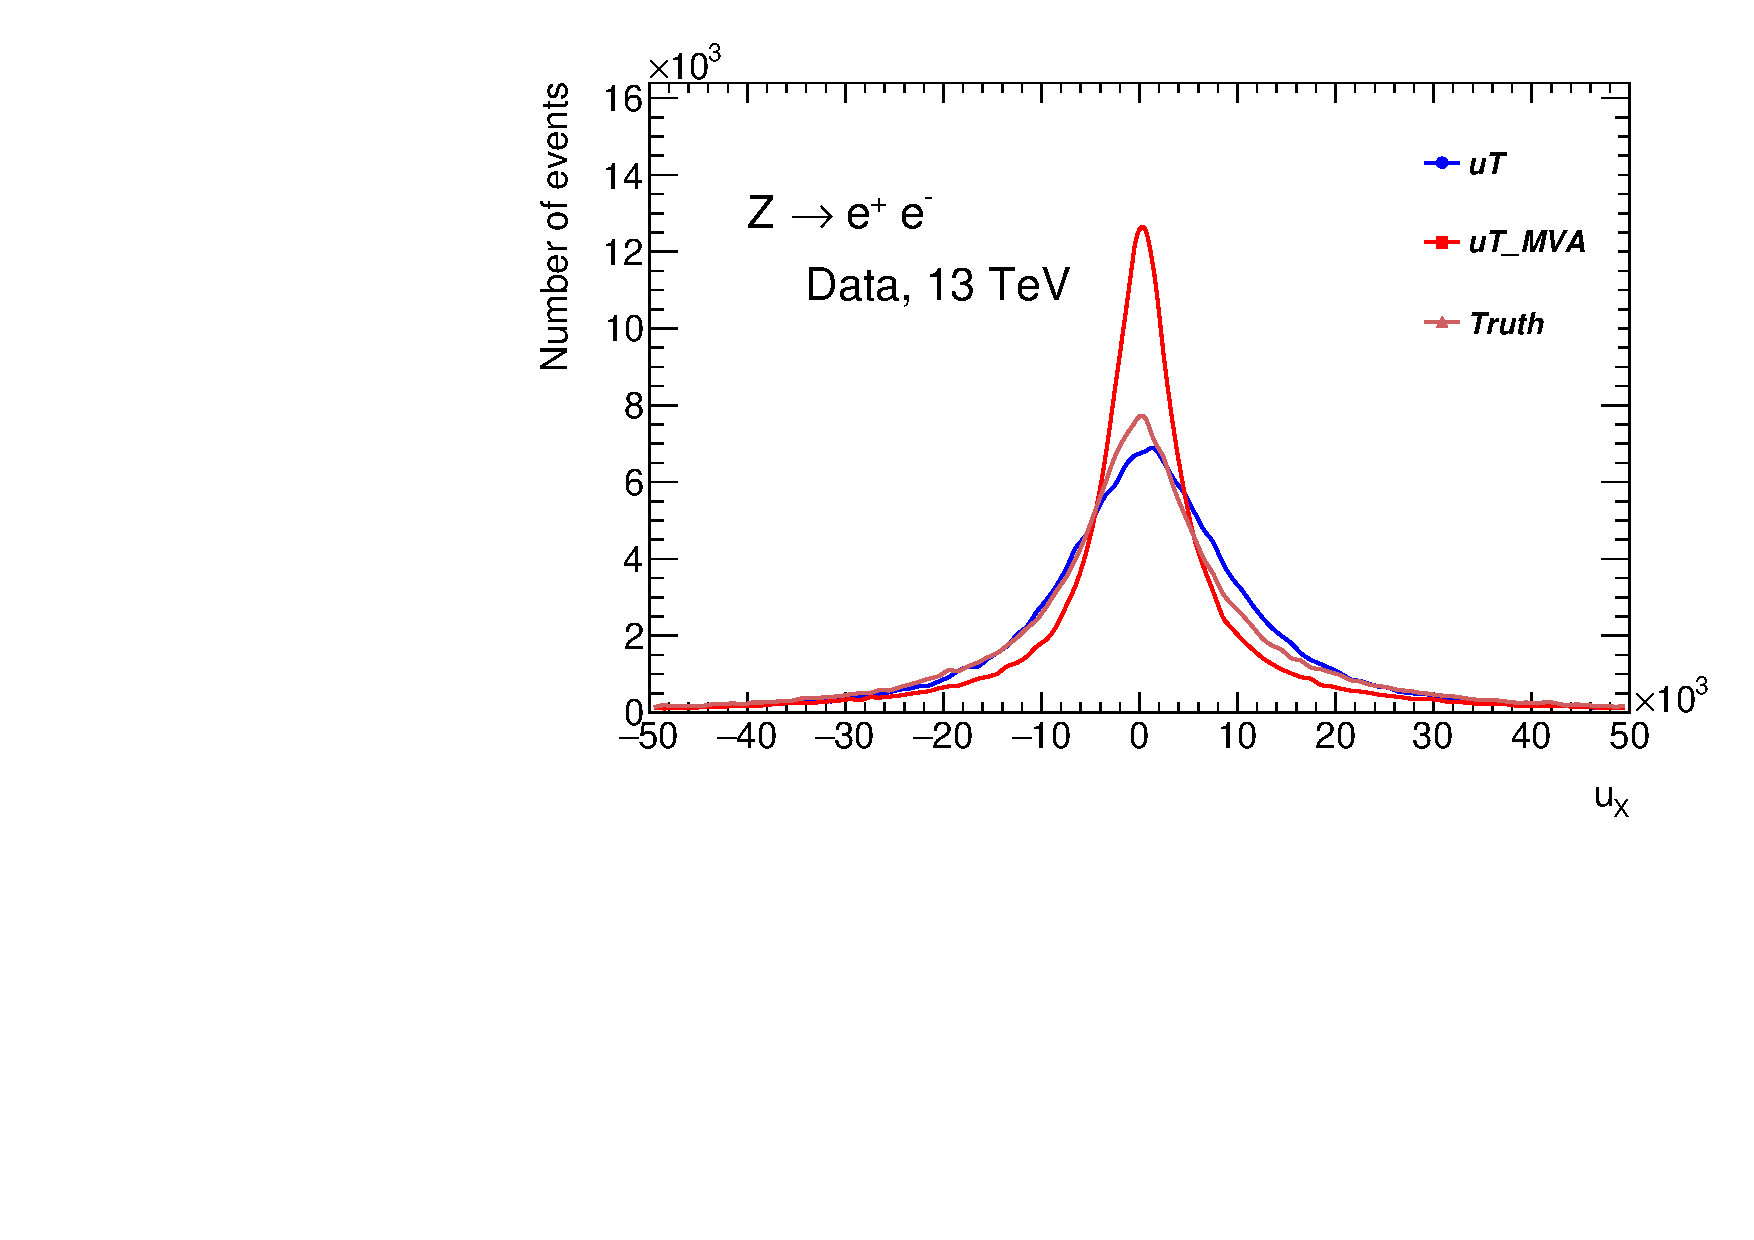
\includegraphics[width=.49\textwidth]{hist_uXzeedata.pdf}}
	{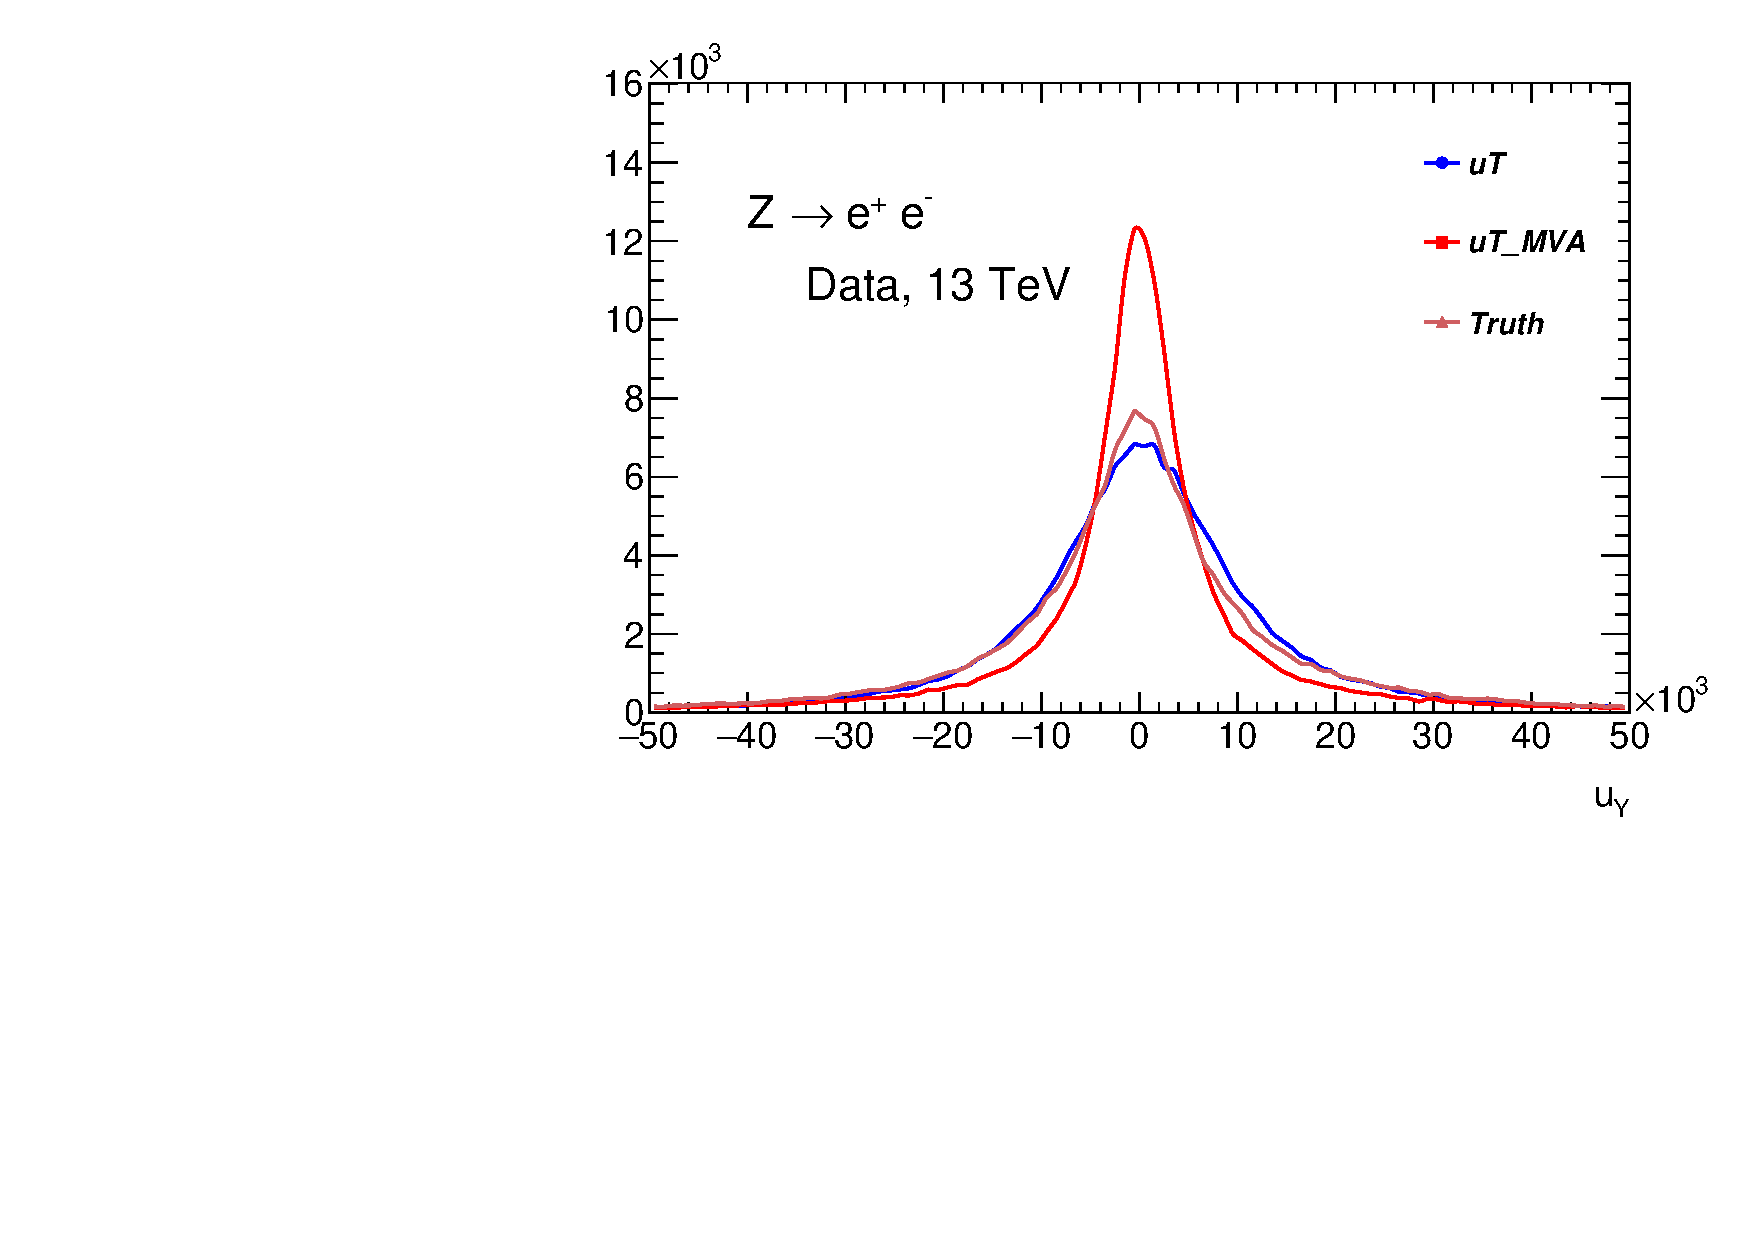
\includegraphics[width=.49\textwidth]{hist_uYzeedata.pdf}} \\
	{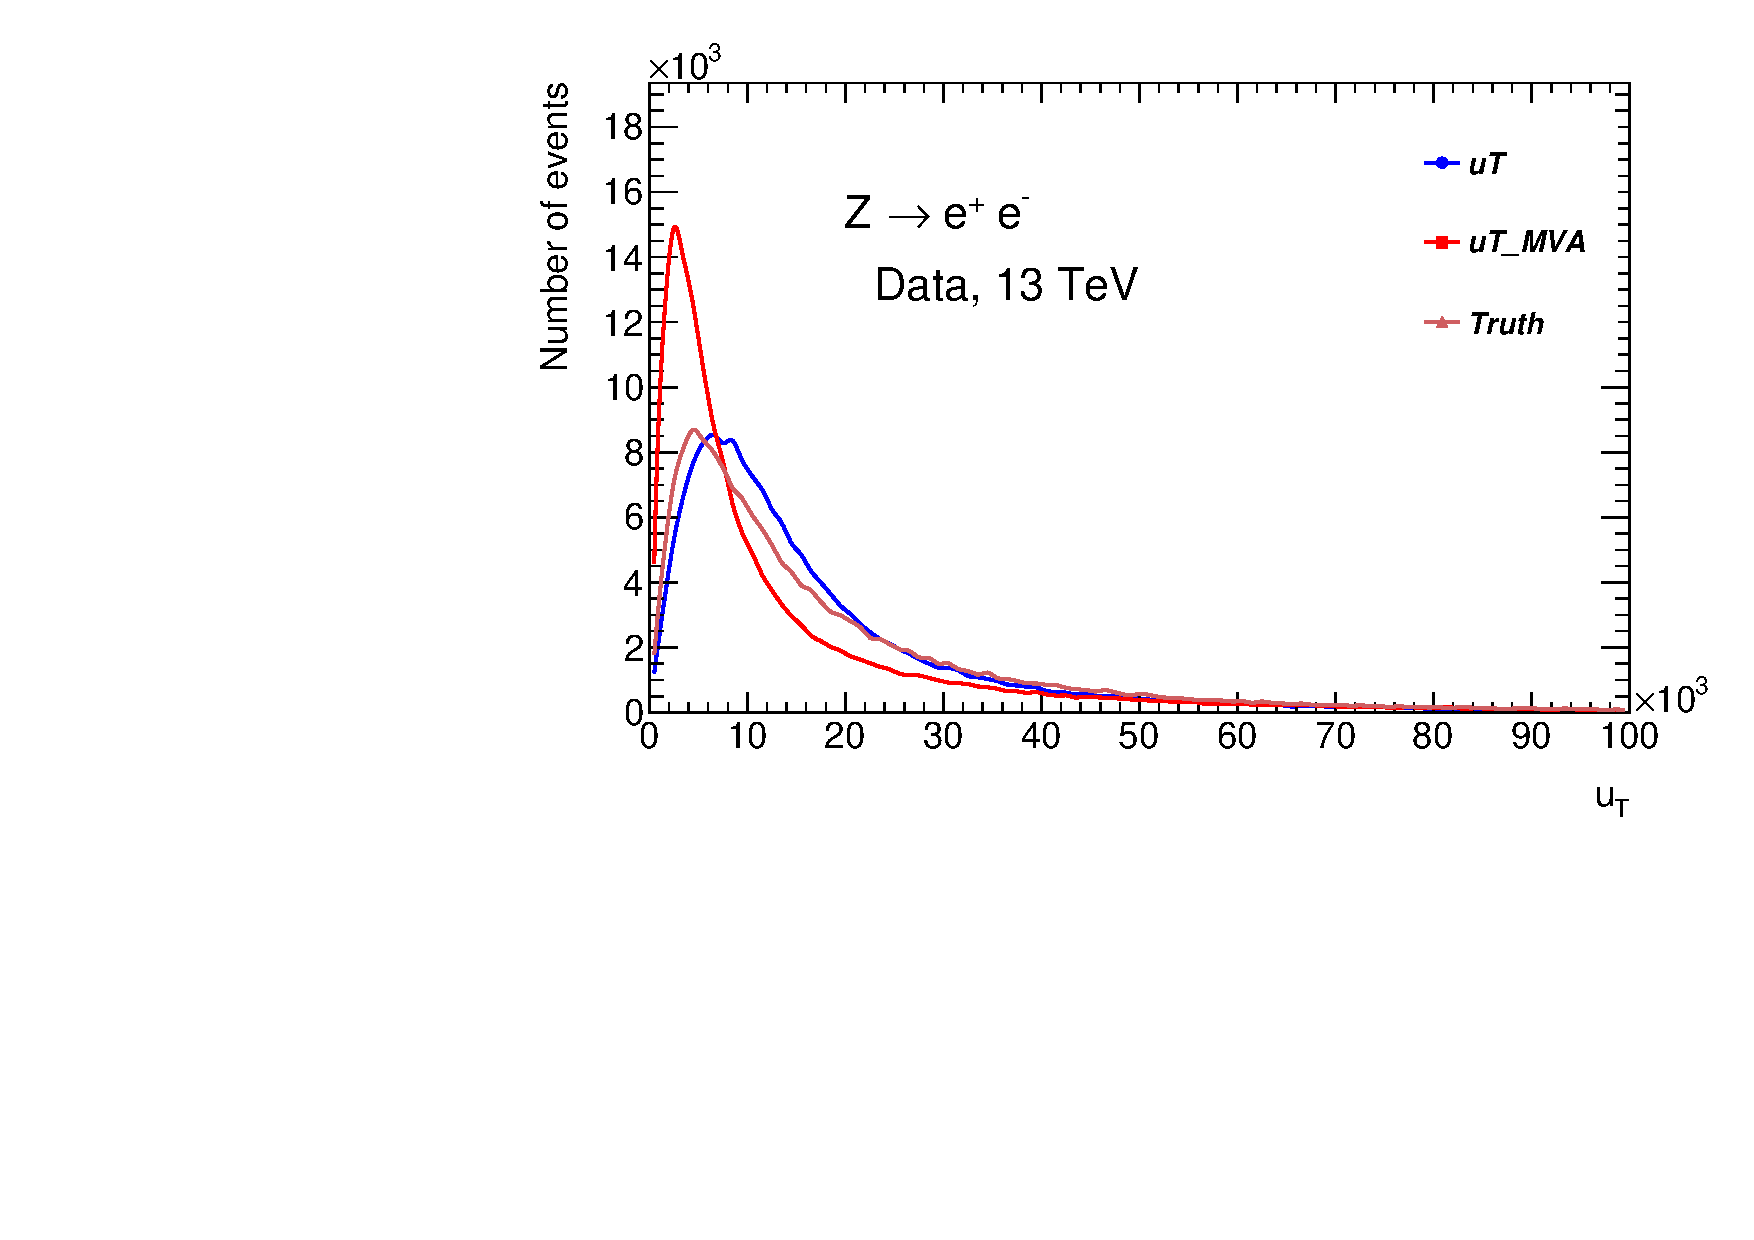
\includegraphics[width=.49\textwidth]{hist_uTzeedata.pdf}}
	{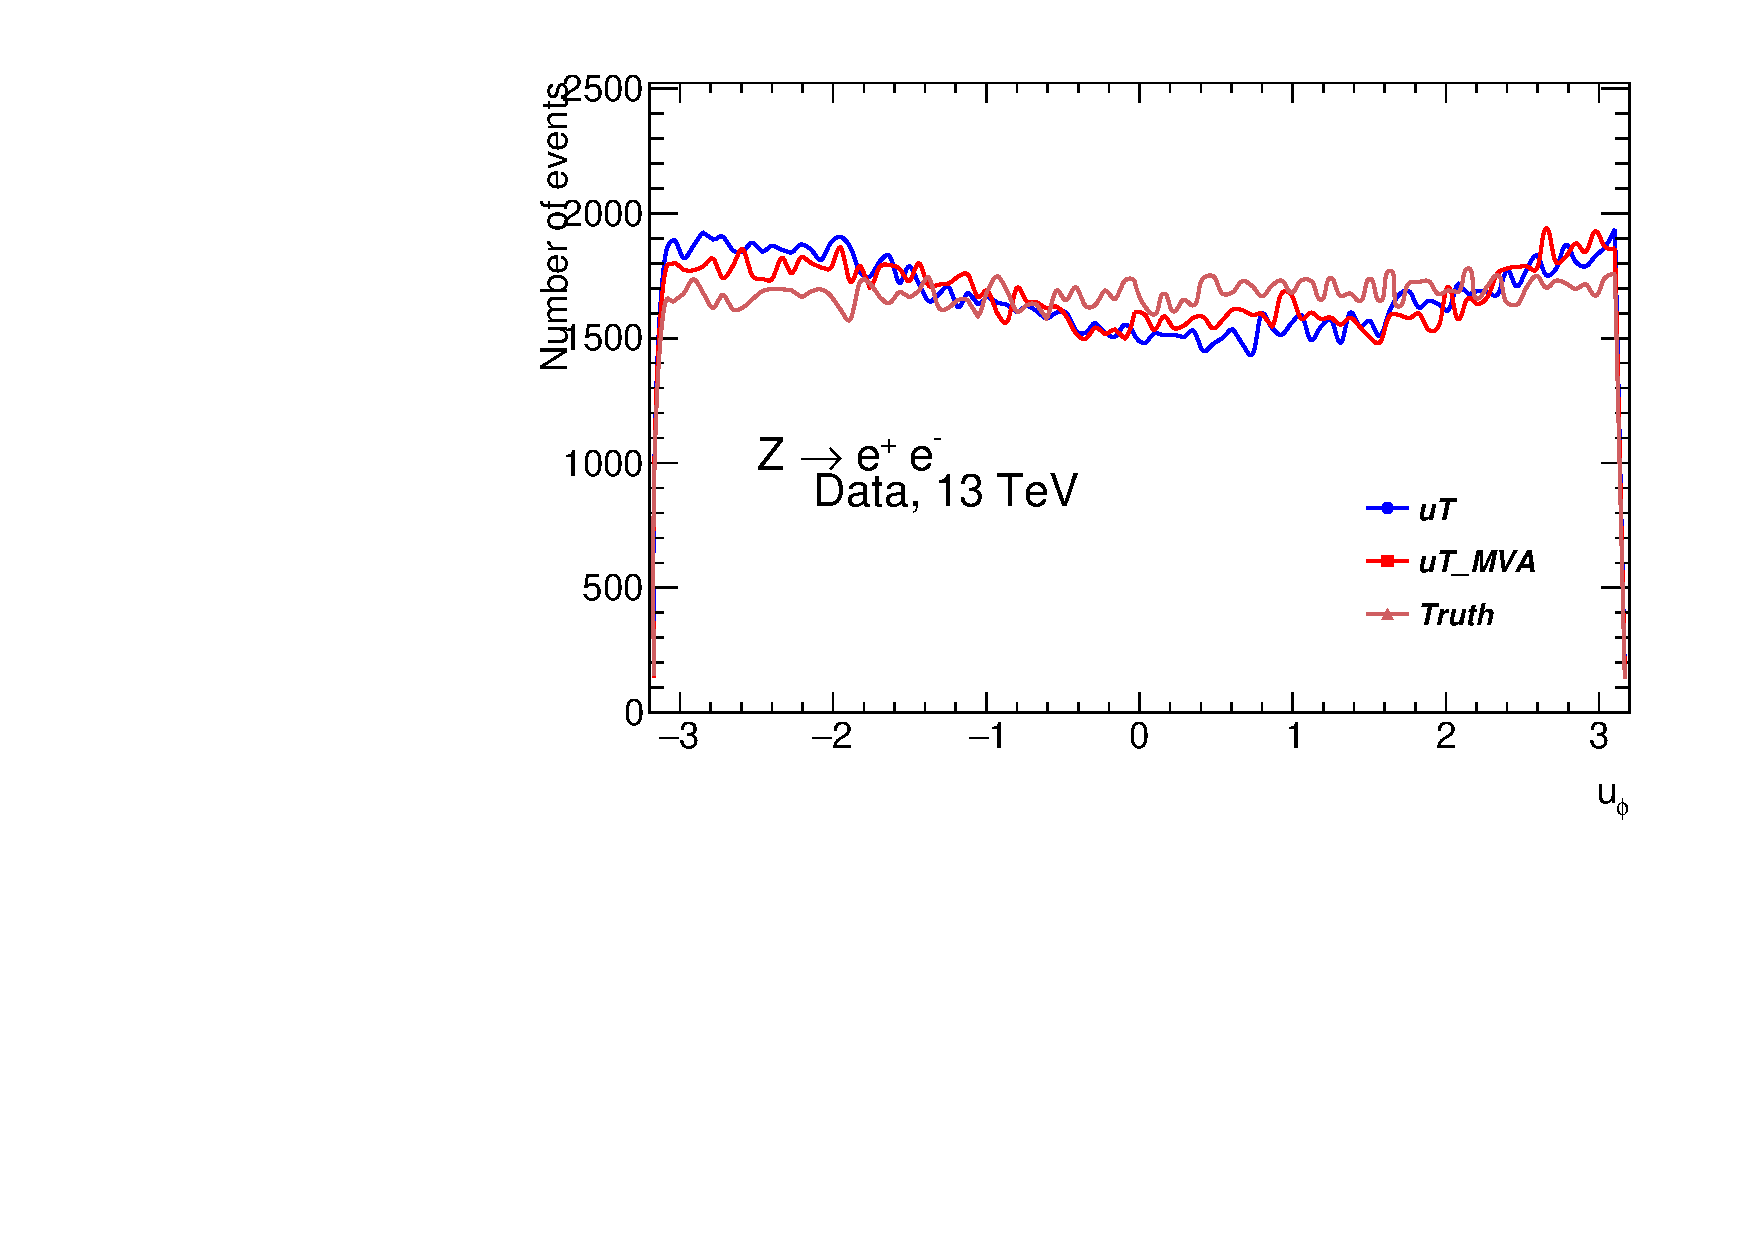
\includegraphics[width=.49\textwidth]{hist_uPhizeedata.pdf}}\\
	{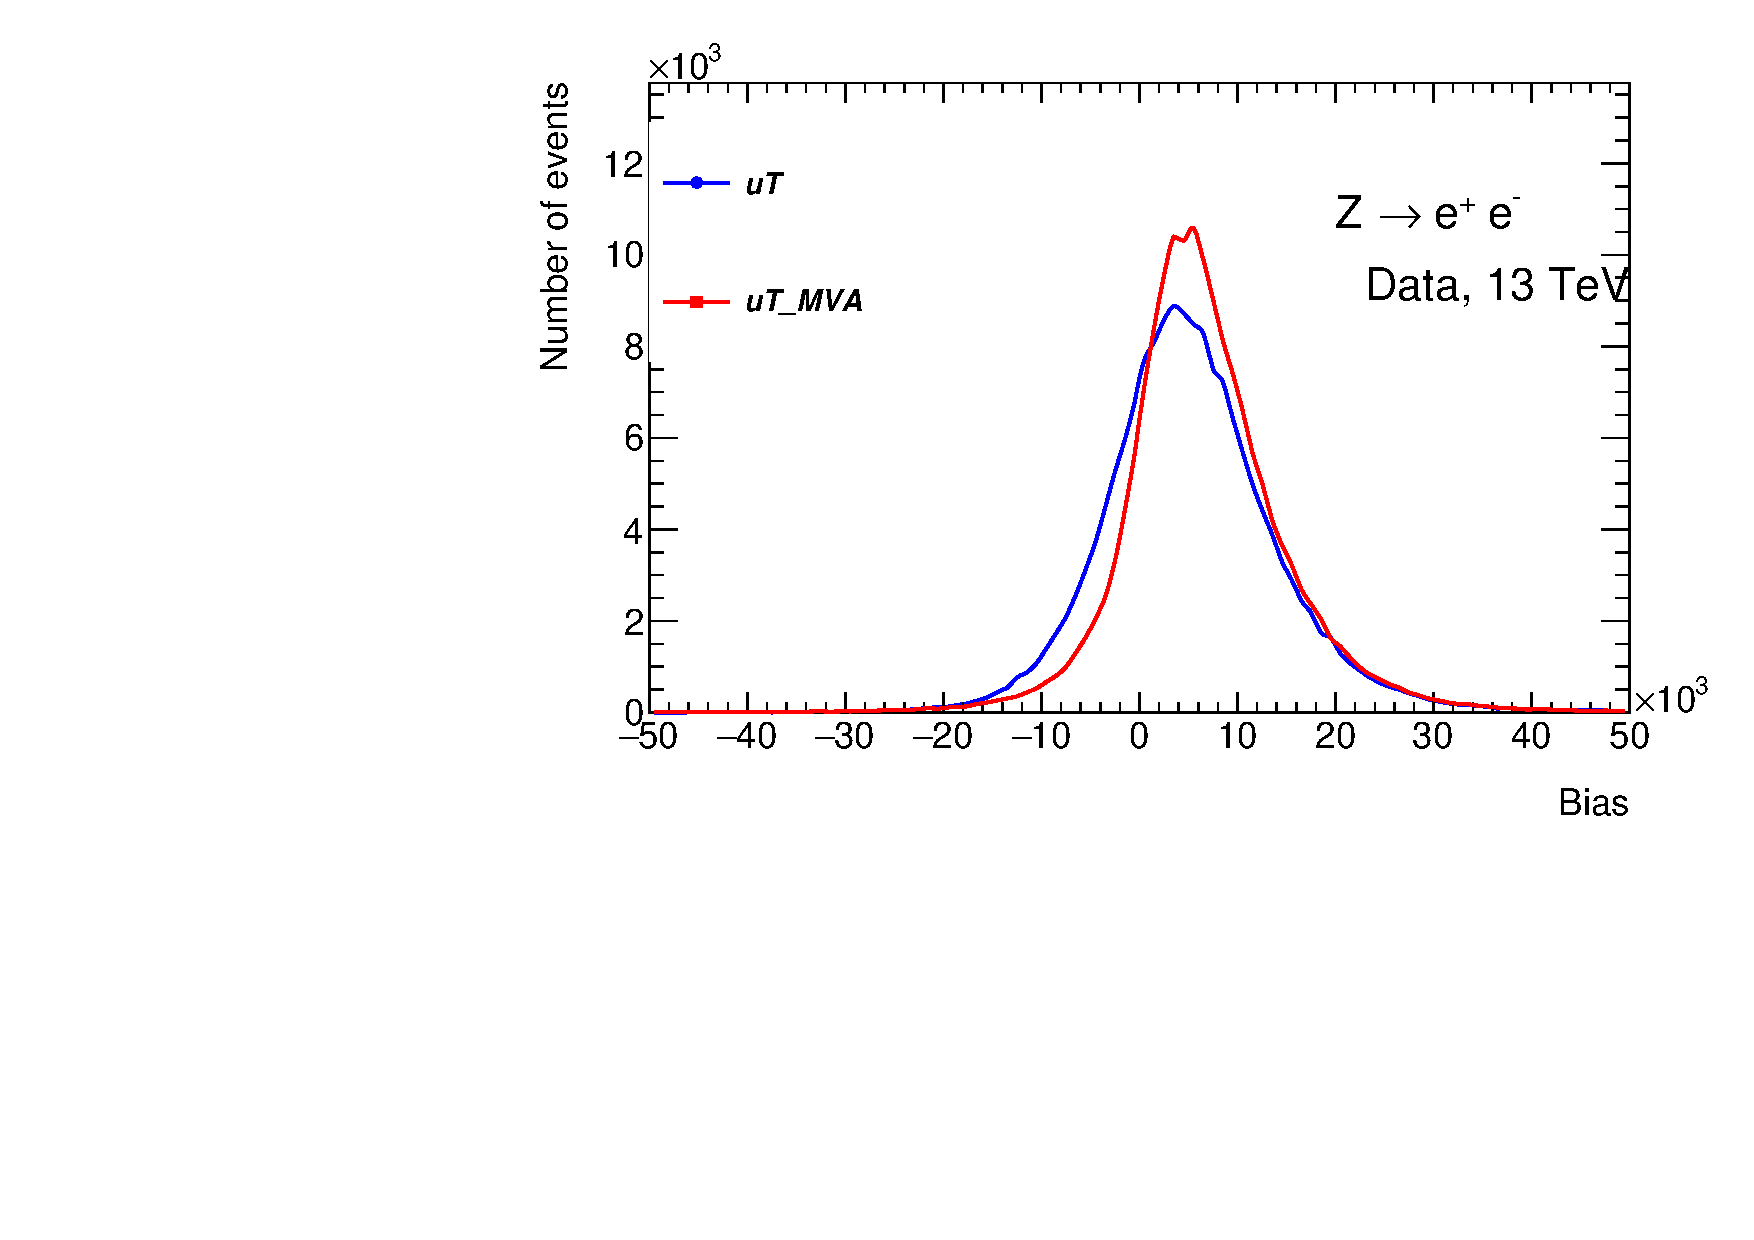
\includegraphics[width=.49\textwidth]{outMVA_biaszeedata.pdf}}
	{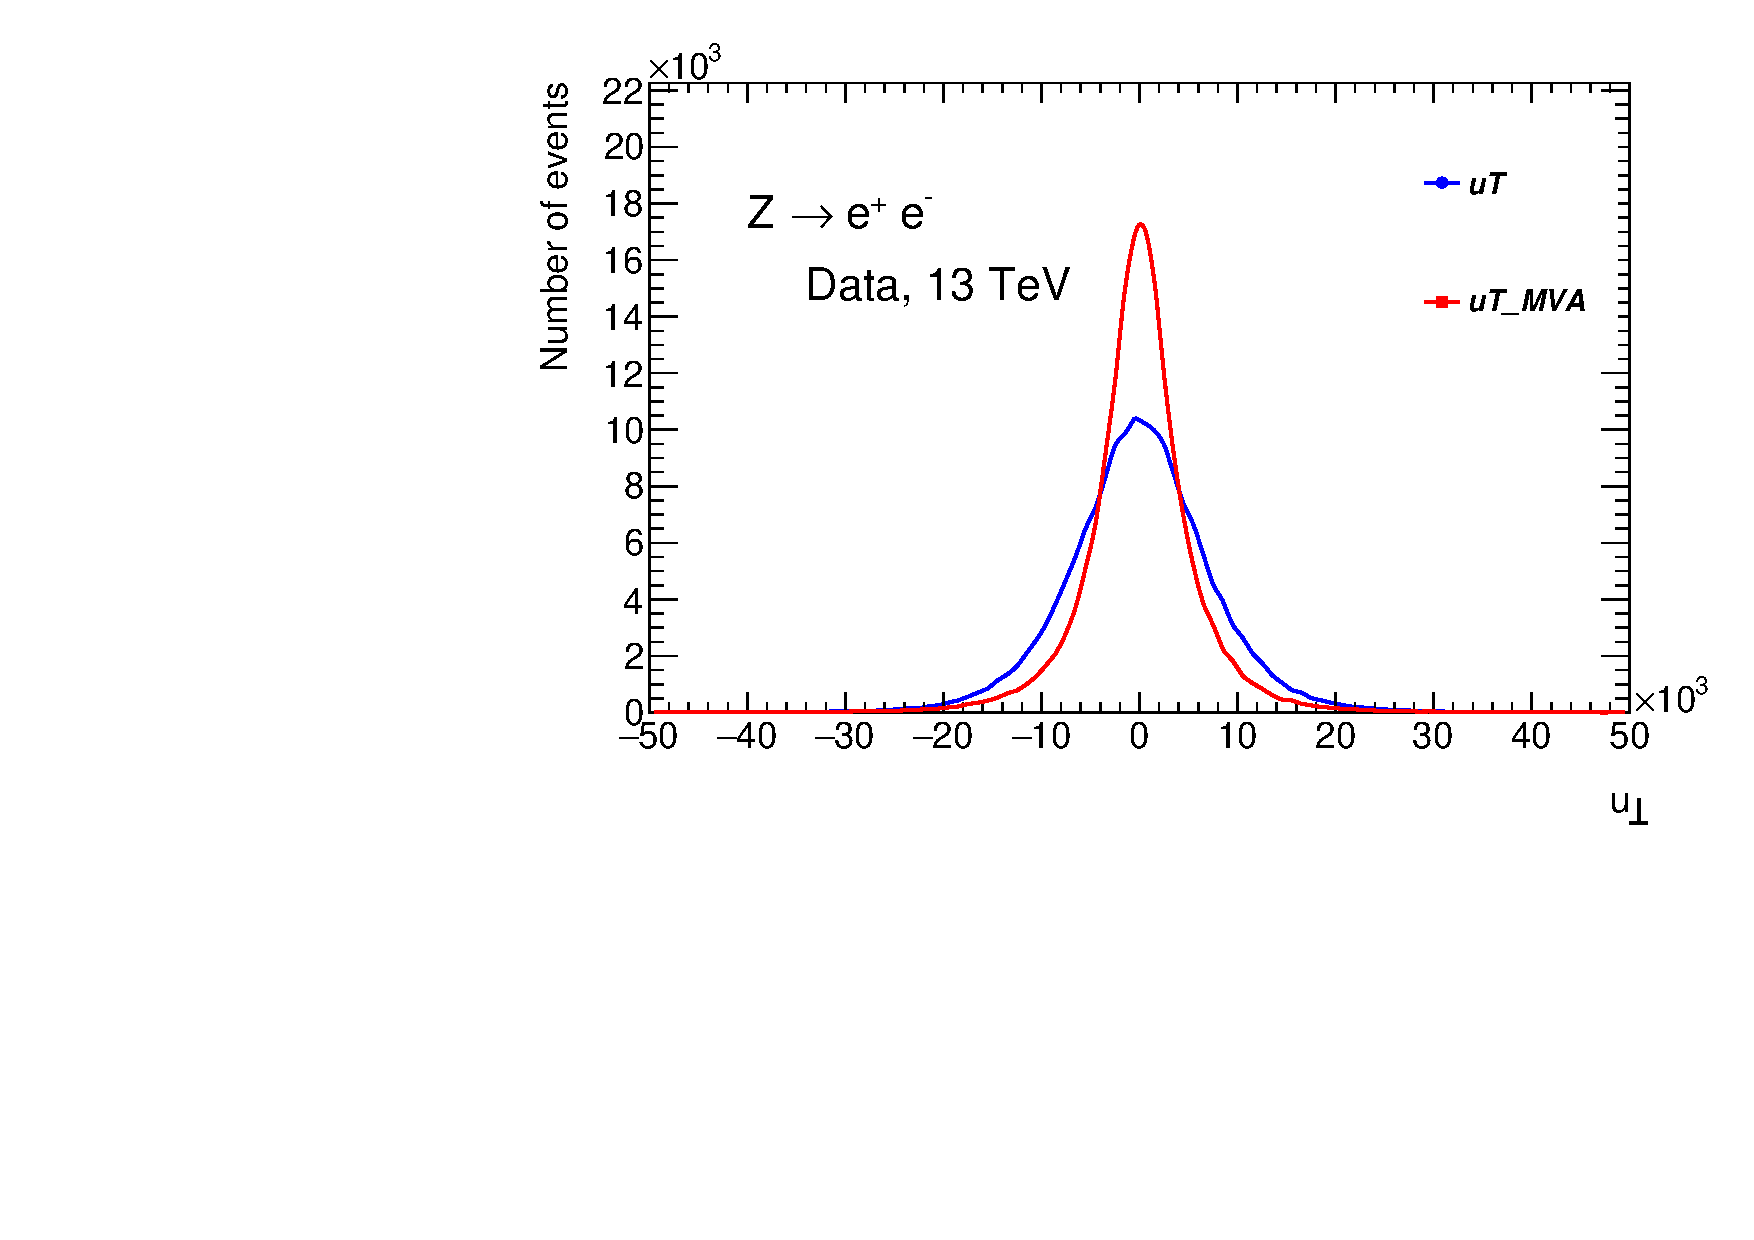
\includegraphics[width=.49\textwidth]{outMVA_uPerpzeedata.pdf}}
	\caption{ Breakdown of systematic uncertainties for 5 (a,b) and 13 (c,d) TeV in the electron channel at the reconstructed level}
	\label{fig:reco_sys_bkd_elec}
\end{figure}
\begin{figure}[h]
	\centering
	{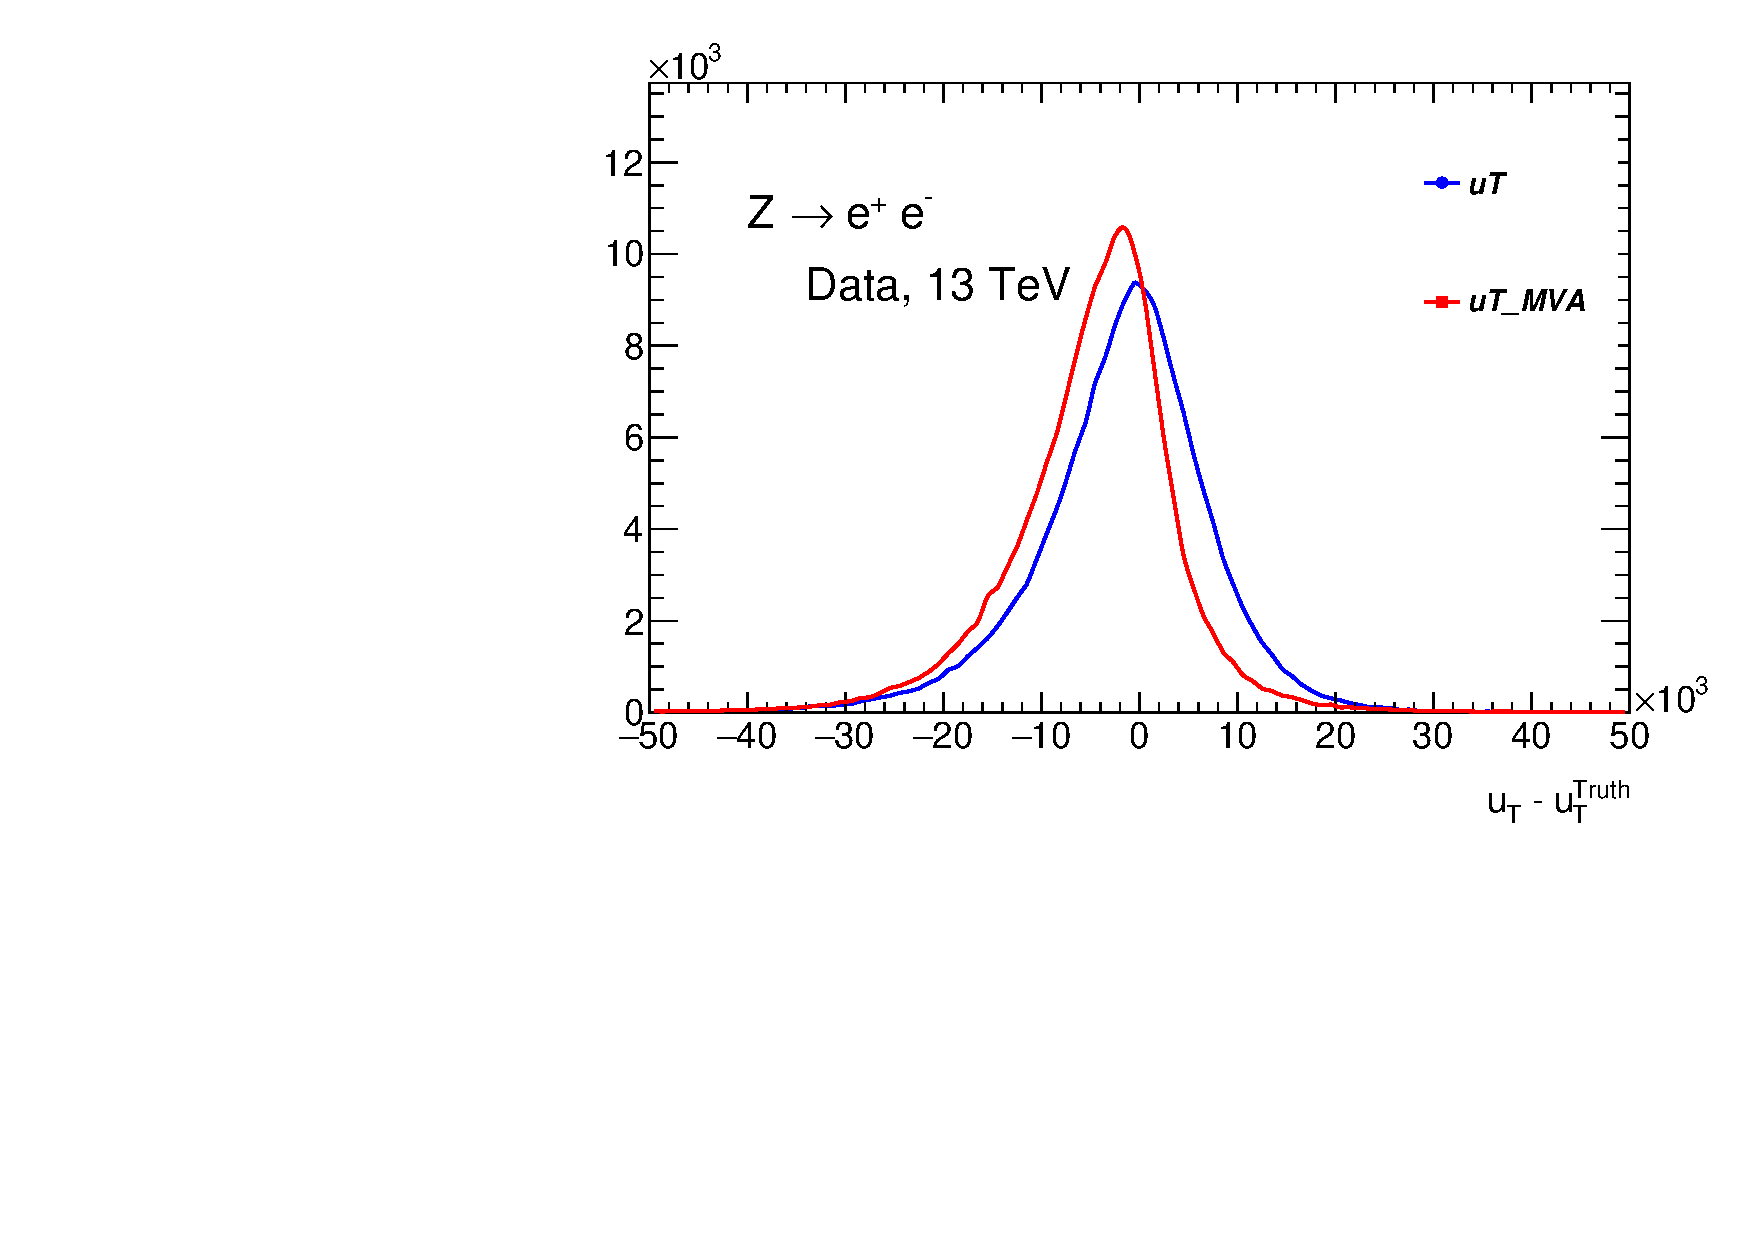
\includegraphics[width=.49\textwidth]{histosDeltaUtzeedata.pdf}}
	{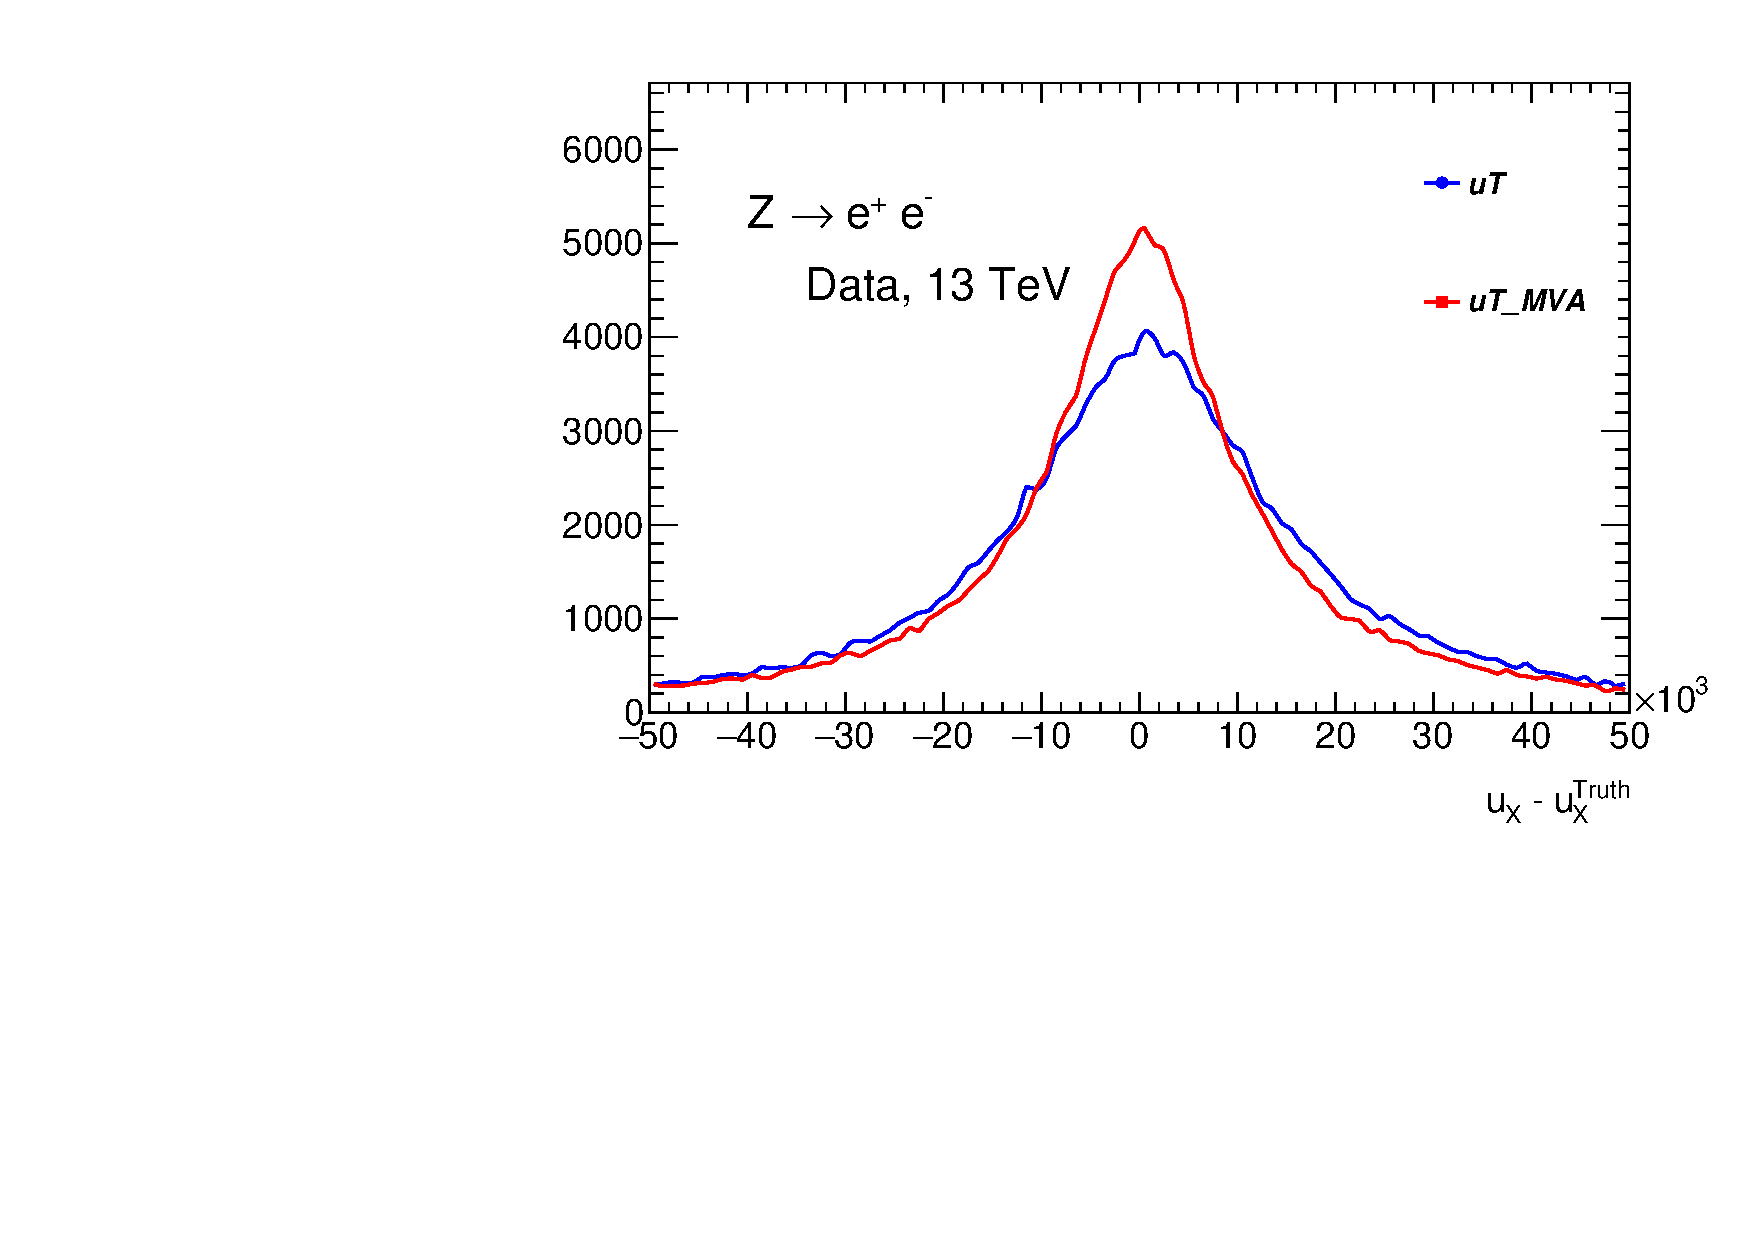
\includegraphics[width=.49\textwidth]{histosDeltaUxzeedata.pdf}} \\
	{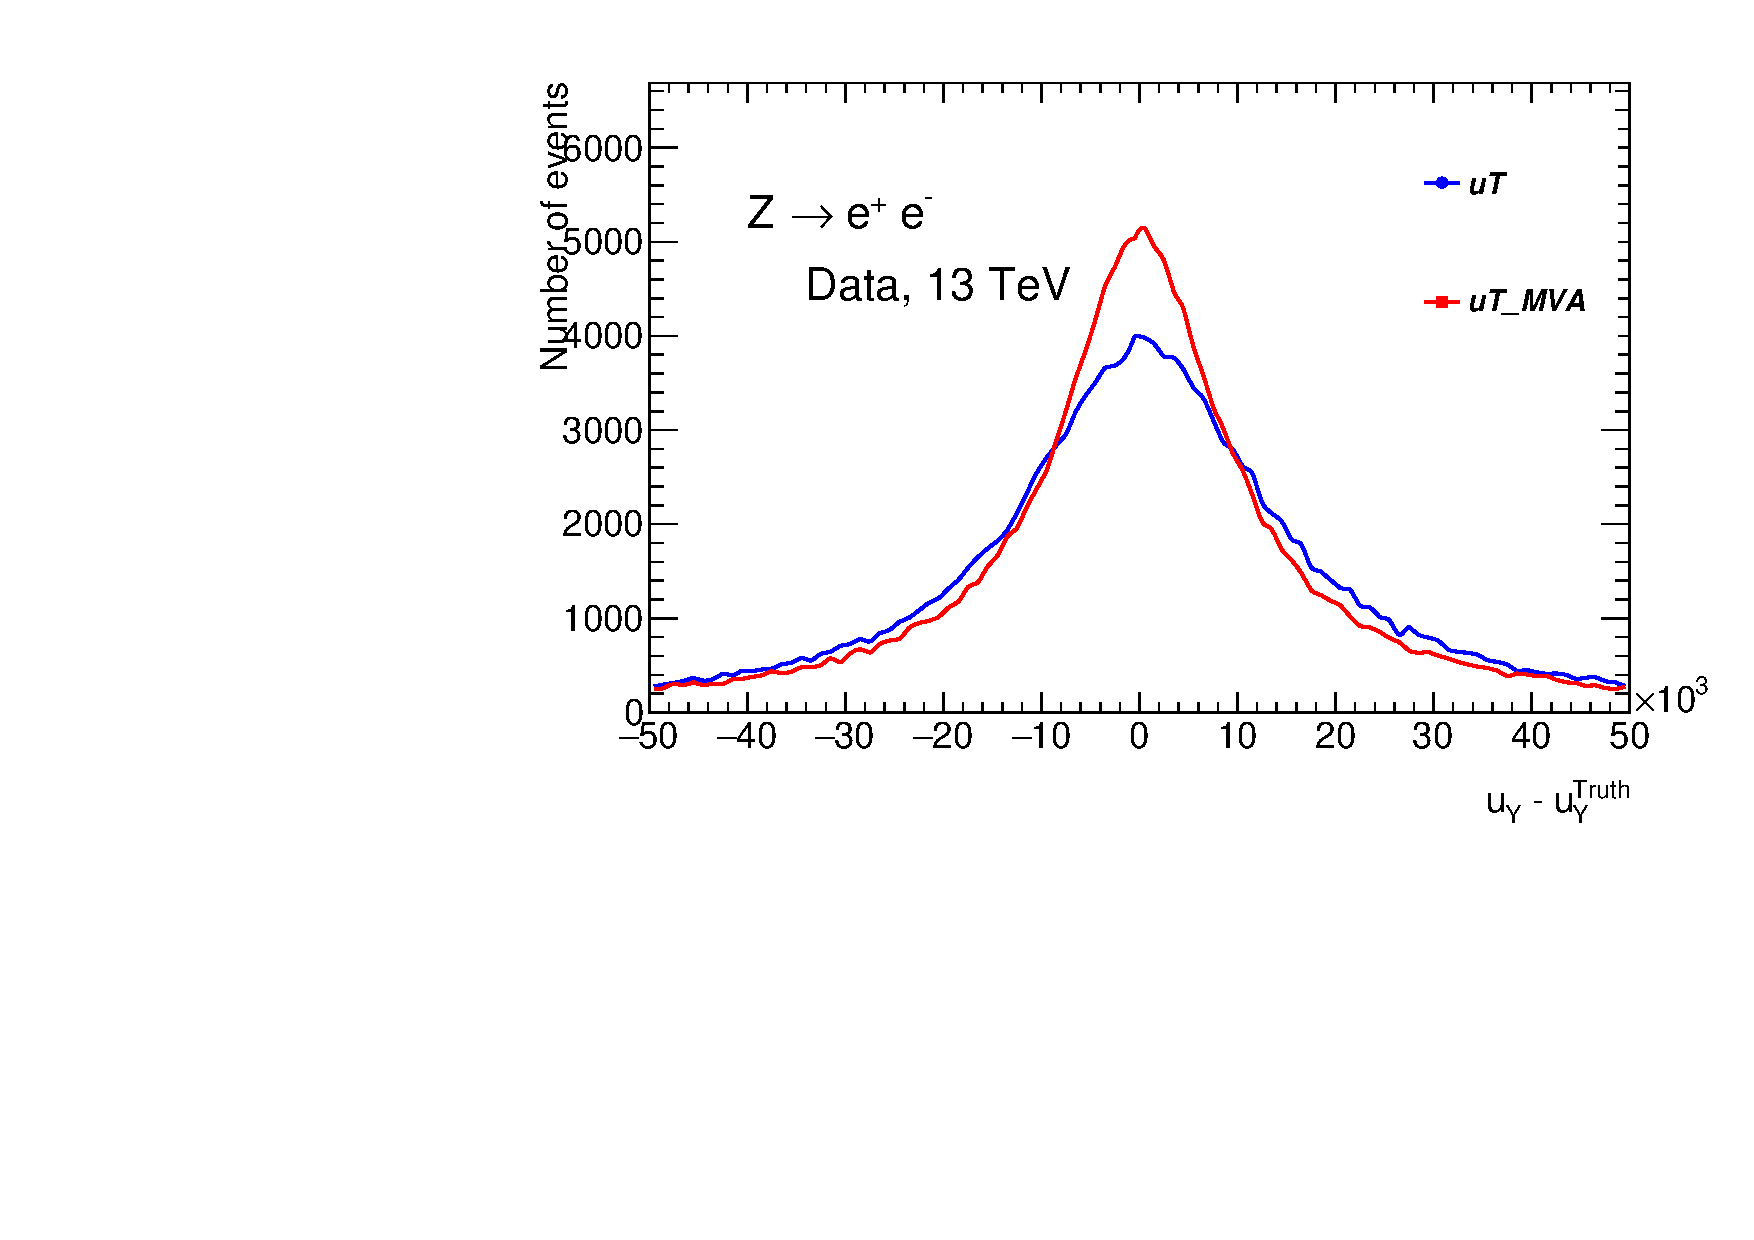
\includegraphics[width=.49\textwidth]{histosDeltaUyzeedata.pdf}}
	{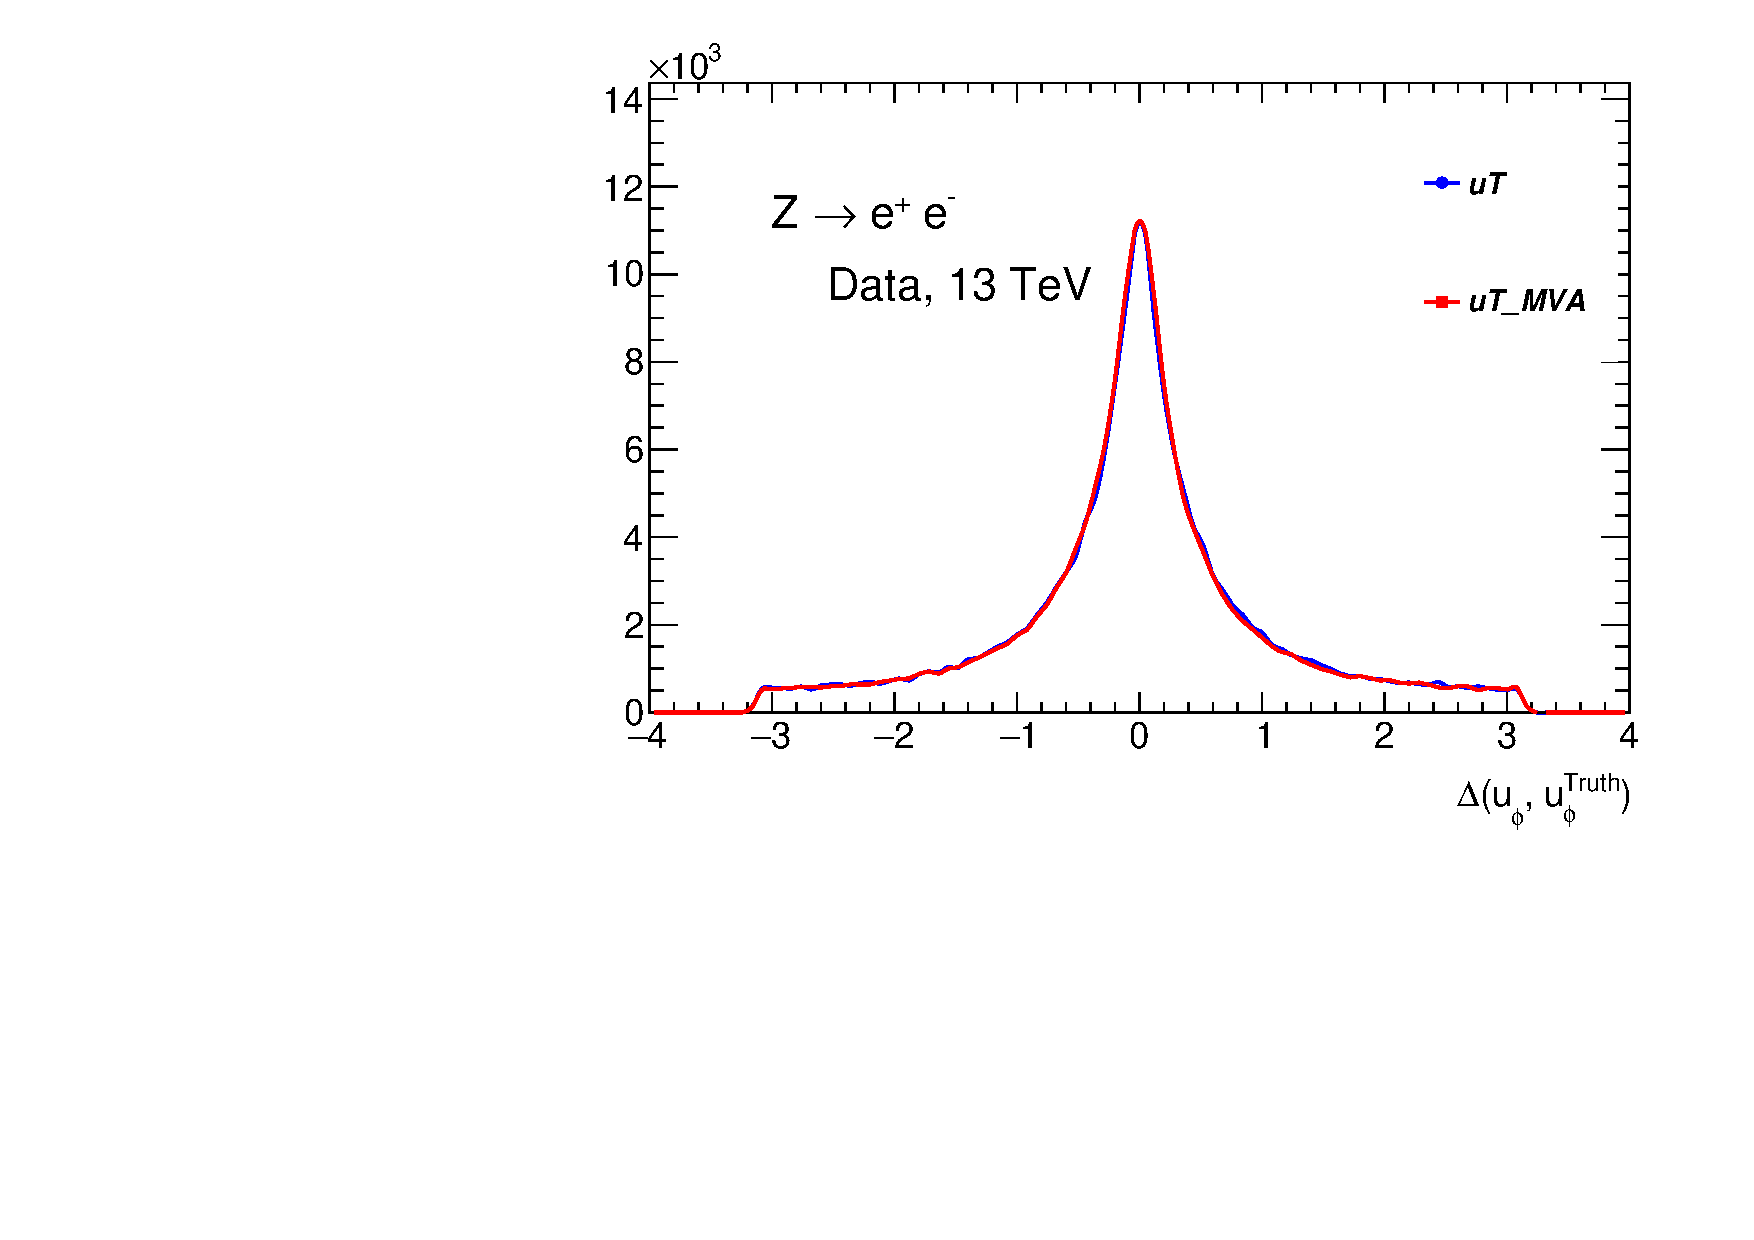
\includegraphics[width=.49\textwidth]{histosDeltaUPhizeedata.pdf}}\\
	{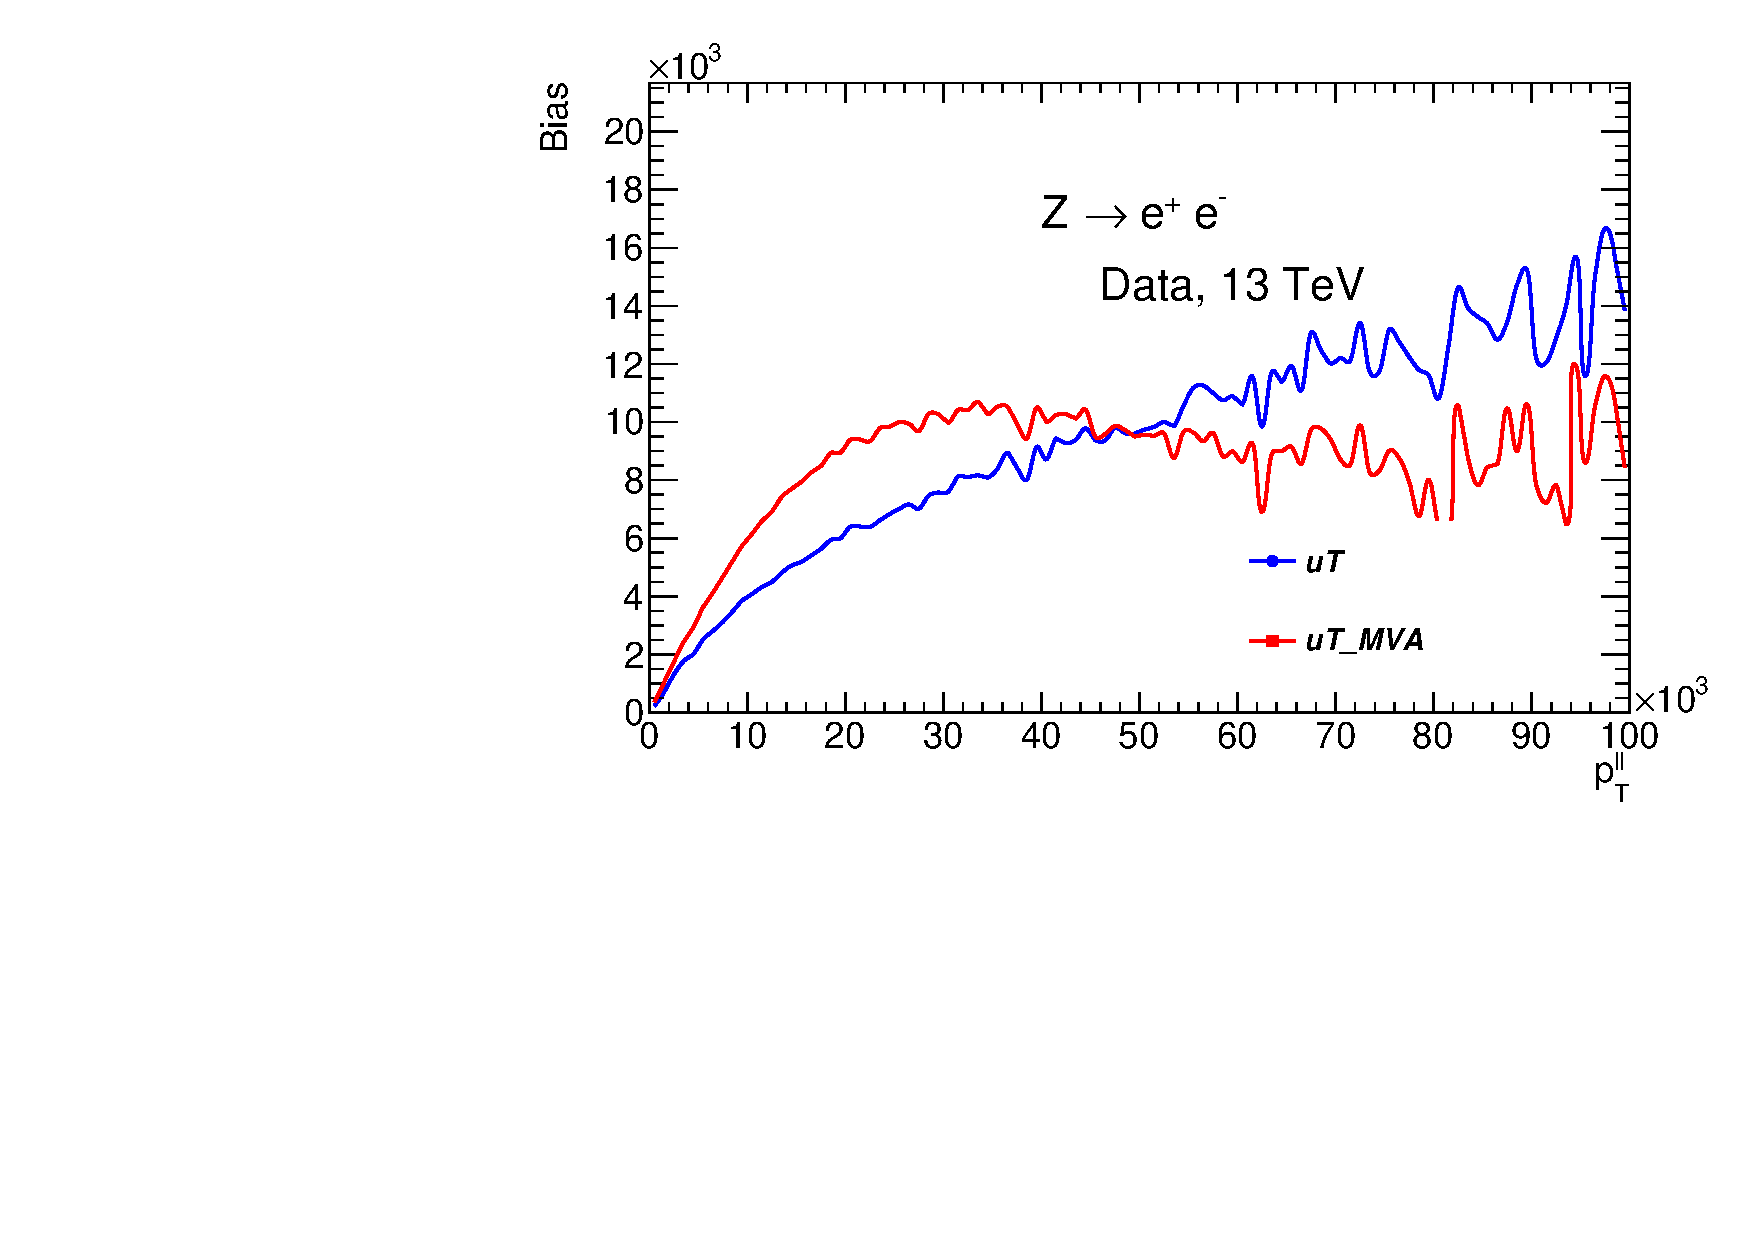
\includegraphics[width=.49\textwidth]{histosMeanBiaszeedata.pdf}}
	{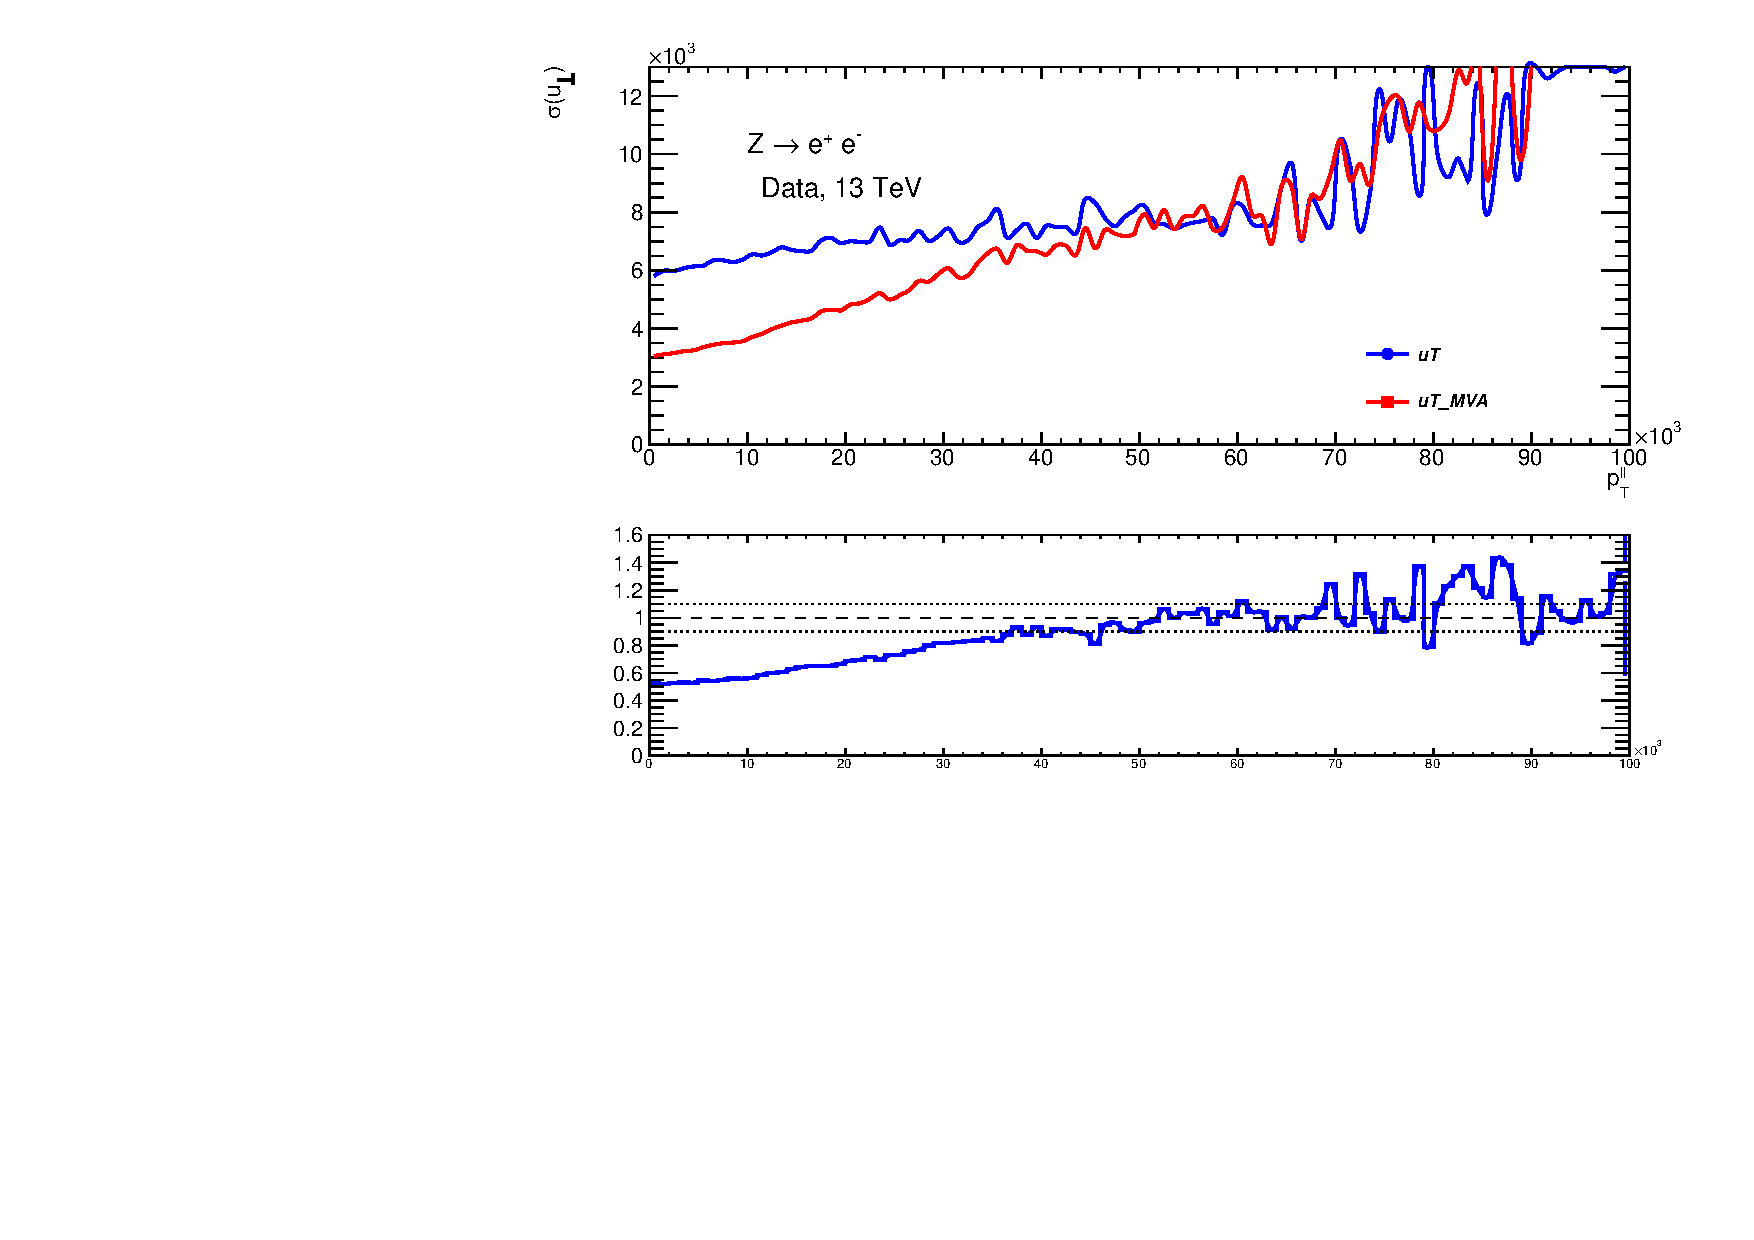
\includegraphics[width=.49\textwidth]{histosSigmaUperpzeedata.pdf}}
	\caption{ Breakdown of systematic uncertainties for 5 (a,b) and 13 (c,d) TeV in the electron channel at the reconstructed level}
	\label{fig:reco_sys_bkd_elec}
\end{figure}
%
%
